\documentclass[tikz,border=0pt]{standalone}
\usepackage{fontspec}
\IfFontExistsTF{TeX Gyre Heros}{\setmainfont{TeX Gyre Heros}}{\setmainfont{Latin Modern Sans}}
\usepackage{amsmath,amssymb,booktabs,array}
\DeclareMathSizes{9}{9}{8.6}{8.6}
\usepackage{pgfplots}
\pgfplotsset{compat=1.17}
\usetikzlibrary{arrows.meta,positioning,calc,fit,shapes.geometric,backgrounds}
\definecolor{ink}{HTML}{183247}
\definecolor{blue}{HTML}{286B91}
\definecolor{teal}{HTML}{19796F}
\definecolor{orange}{HTML}{AC671F}
\definecolor{muted}{HTML}{596C78}
\tikzset{
  every node/.style={font=\fontsize{9}{11}\selectfont,text=ink},
  arr/.style={-{Stealth[length=1.7mm]},line width=.55pt,draw=muted},
  panel/.style={draw=muted!35,line width=.5pt,rounded corners=1mm,fill=white},
  box/.style={draw=blue!70,line width=.55pt,rounded corners=.8mm,fill=blue!5,align=center,inner sep=2mm},
  label/.style={font=\fontsize{9}{11}\selectfont,align=left,inner sep=0},
  paneltitle/.style={font=\bfseries\fontsize{9.5}{12}\selectfont,anchor=west,inner sep=0}
}

\begin{document}
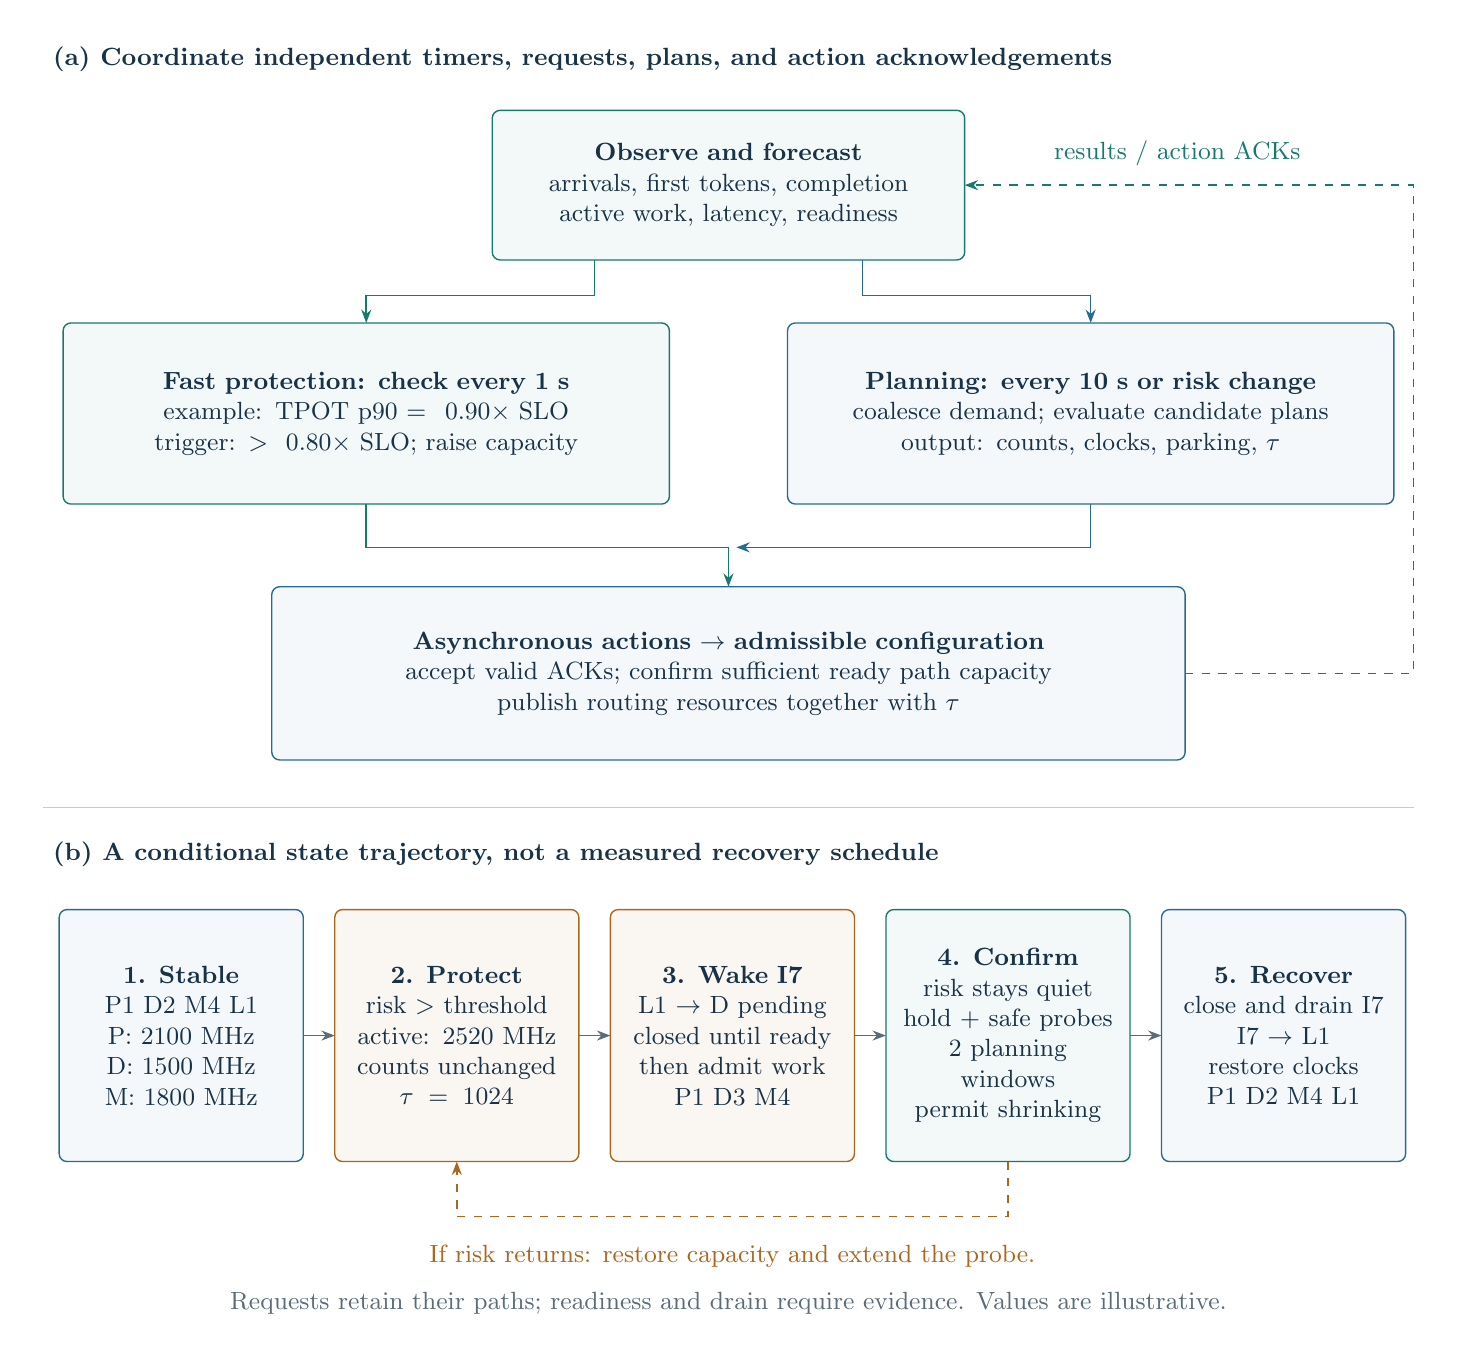
\begin{tikzpicture}[x=1mm,y=-1mm,font=\fontsize{9}{11}\selectfont]
  \path[use as bounding box] (0,0) rectangle (178,164);
  \node[anchor=west,font=\bfseries\fontsize{9}{11}\selectfont,text=ink] at (2,4) {(a) Coordinate independent timers, requests, plans, and action acknowledgements};

  \node[panel,draw=teal,fill=teal!5,minimum width=60mm,minimum height=19mm,align=center,text width=56mm] (observe) at (89,20) {\textbf{Observe and forecast}\\arrivals, first tokens, completion\\active work, latency, readiness};

  \node[panel,draw=teal,fill=teal!5,minimum width=77mm,minimum height=23mm,align=center,text width=73mm] (fast) at (43,49) {\textbf{Fast protection: check every 1 s}\\example: TPOT p90 $=0.90\times$ SLO\\trigger: $>0.80\times$ SLO; raise capacity};
  \node[panel,draw=blue,fill=blue!5,minimum width=77mm,minimum height=23mm,align=center,text width=73mm] (slow) at (135,49) {\textbf{Planning: every 10 s or risk change}\\coalesce demand; evaluate candidate plans\\output: counts, clocks, parking, $\tau$};
  \draw[arr,draw=teal] (72,29.5) -- (72,34) -- (43,34) -- (43,37.5);
  \draw[arr,draw=blue] (106,29.5) -- (106,34) -- (135,34) -- (135,37.5);
  \draw[arr,draw=teal] (43,60.5) -- (43,66) -- (89,66) -- (89,71);
  \draw[arr,draw=blue] (135,60.5) -- (135,66) -- (90,66);

  \node[panel,draw=blue,fill=blue!5,minimum width=116mm,minimum height=22mm,align=center,text width=112mm] (publish) at (89,82) {\textbf{Asynchronous actions $\rightarrow$ admissible configuration}\\accept valid ACKs; confirm sufficient ready path capacity\\publish routing resources together with $\tau$};
  \draw[arr,draw=teal,dashed] (147,82) -- (176,82) -- (176,20) -- (119,20);
  \node[fill=white,inner sep=0.5mm,text=teal] at (146,16) {results / action ACKs};

  \draw[muted!35] (2,99) -- (176,99);
  \node[anchor=west,font=\bfseries\fontsize{9}{11}\selectfont,text=ink] at (2,105) {(b) A conditional state trajectory, not a measured recovery schedule};

  \node[panel,draw=blue,fill=blue!5,minimum width=31mm,minimum height=32mm,align=center,text width=28mm] at (19.5,128) {\textbf{1. Stable}\\P1 D2 M4 L1\\P: 2100 MHz\\D: 1500 MHz\\M: 1800 MHz};
  \node[panel,draw=orange,fill=orange!6,minimum width=31mm,minimum height=32mm,align=center,text width=28mm] at (54.5,128) {\textbf{2. Protect}\\risk $>$ threshold\\active: 2520 MHz\\counts unchanged\\$\tau=1024$};
  \node[panel,draw=orange,fill=orange!6,minimum width=31mm,minimum height=32mm,align=center,text width=28mm] at (89.5,128) {\textbf{3. Wake I7}\\L1 $\rightarrow$ D pending\\closed until ready\\then admit work\\P1 D3 M4};
  \node[panel,draw=teal,fill=teal!5,minimum width=31mm,minimum height=32mm,align=center,text width=28mm] at (124.5,128) {\textbf{4. Confirm}\\risk stays quiet\\hold + safe probes\\2 planning windows\\permit shrinking};
  \node[panel,draw=blue,fill=blue!5,minimum width=31mm,minimum height=32mm,align=center,text width=28mm] at (159.5,128) {\textbf{5. Recover}\\close and drain I7\\I7 $\rightarrow$ L1\\restore clocks\\P1 D2 M4 L1};
  \foreach \a/\b in {35/39,70/74,105/109,140/144} {\draw[arr] (\a,128) -- (\b,128);}

  \draw[arr,draw=orange,dashed] (124.5,144) -- (124.5,151) -- (54.5,151) -- (54.5,144);
  \node[fill=white,inner sep=0.5mm,text=orange] at (89.5,156) {If risk returns: restore capacity and extend the probe.};
  \node[text=muted] at (89,162) {Requests retain their paths; readiness and drain require evidence. Values are illustrative.};
\end{tikzpicture}
\end{document}
